\documentclass[letterpaper,11pt]{article}
\usepackage[english]{babel}
\usepackage[utf8x]{inputenc}
\usepackage{apacite}
\usepackage[left=2cm,top=2cm,right=2cm,bottom=1.5cm,head=.5cm,foot=.5cm]{geometry}
\usepackage{graphicx}
\usepackage{amsmath}
\usepackage{hyperref}
\usepackage{cite}
\usepackage{xr-hyper}
\usepackage{float}
\usepackage{xr} 
\usepackage{adjustbox}
\usepackage{url}
\usepackage{multirow}
\usepackage{longtable}
\usepackage{subfig}
\usepackage{float}
\usepackage{setspace}
\usepackage{lineno}
\usepackage{natbib}
\usepackage{amsmath}
\usepackage{authblk}
\usepackage{xr}
\usepackage{relsize}
\usepackage{tikz}


%%%% HELPER CODE FOR DEALING WITH EXTERNAL REFERENCES
% (from an answer by cyberSingularity at http://tex.stackexchange.com/a/69832/226)
%%%

\usepackage{xcite}

\usepackage{xr}
\makeatletter
\renewcommand \thesection{S\@arabic\c@section}
\renewcommand\thetable{S\@arabic\c@table}
\renewcommand \thefigure{S\@arabic\c@figure}
\makeatother
\newcommand*{\addFileDependency}[1]{% argument=file name and extension
  \typeout{(#1)}% latexmk will find this if $recorder=0 (however, in that case, it will ignore #1 if it is a .aux or .pdf file etc and it exists! if it doesn't exist, it will appear in the list of dependents regardless)
  \@addtofilelist{#1}% if you want it to appear in \listfiles, not really necessary and latexmk doesn't use this
  \IfFileExists{#1}{}{\typeout{No file #1.}}% latexmk will find this message if #1 doesn't exist (yet)
}
\makeatother

\newcommand*{\myexternaldocument}[1]{%
    \externaldocument{#1}%
    \addFileDependency{#1.tex}%
    \addFileDependency{#1.aux}%
}
%%% END HELPER CODE

% put all the external documents here!
%\myexternaldocument{SI}

\title{Supplementary Materials to Harnessing Machine Learning to Identify Antimicrobial Peptides in \textit{Drosophila melanogaster}}
\author[a,*]{Nilanjan Roy}
\date{}
\affil[a]{Department of Molecular Biosciences, University of Kansas}
\affil[*]{Corresponding author: nilanjan.roy@ku.edu}

\begin{document}

\maketitle

%\section{Supplementary Materials}

\begin{figure}[H]
    \centering
    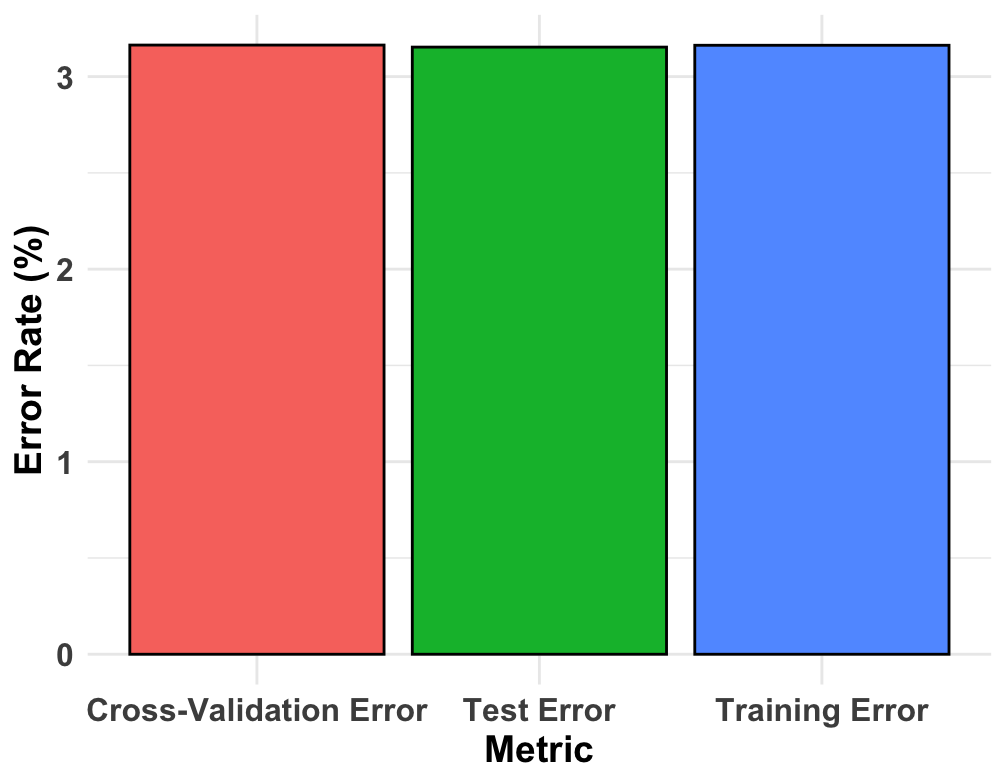
\includegraphics[width=1\textwidth]{figures/Random_forest_error_rate.png}
    \caption{Error rate in the Random forest model}
    \label{fig:Random_forest_error_rate}
\end{figure}

\begin{figure}[H]
    \centering
    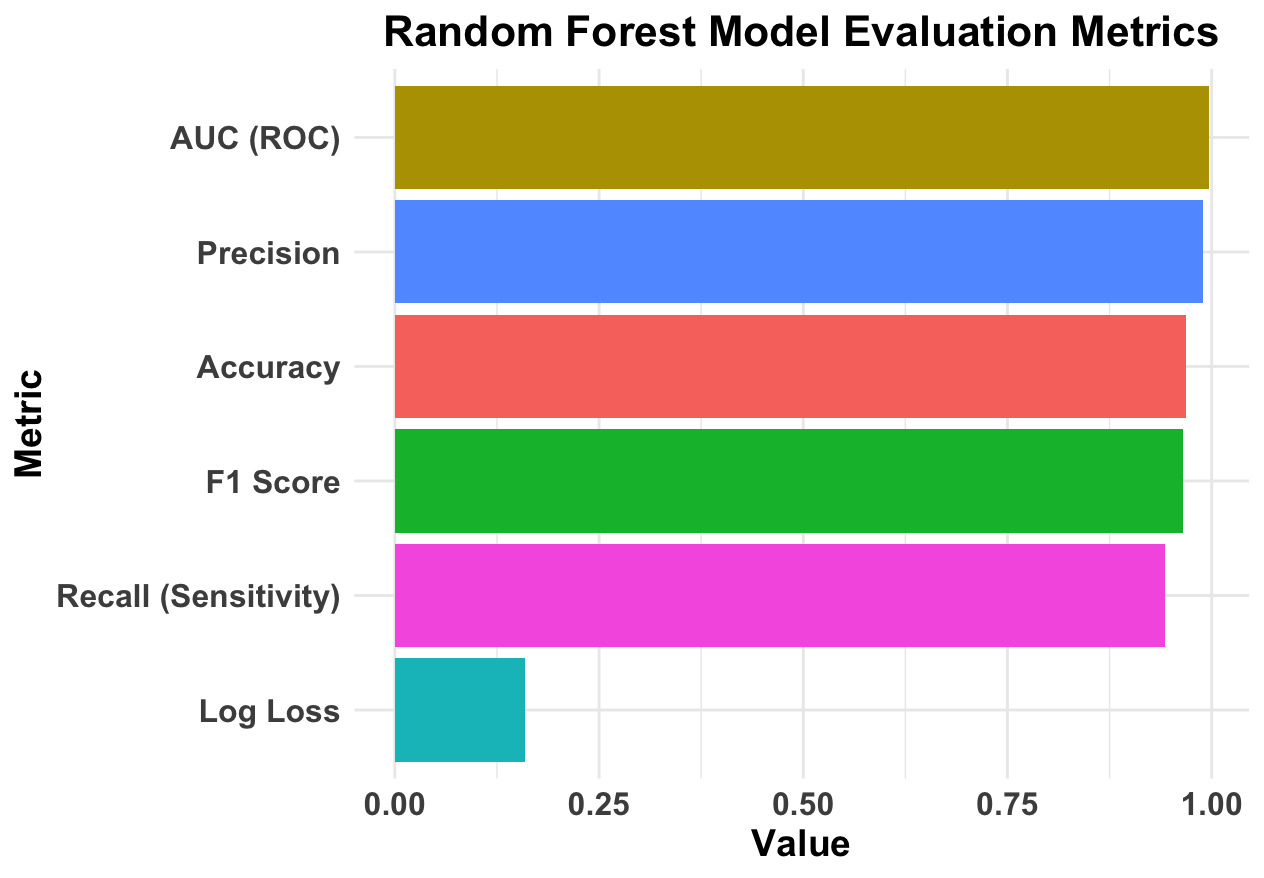
\includegraphics[width=0.7\textwidth]{figures/Random_forest_evaluation_matrices.jpg}
    \caption{Different evaluation matrices of the Random forest model}
    \label{fig:featureimportance}
\end{figure}

\begin{figure}[H]
    \centering
    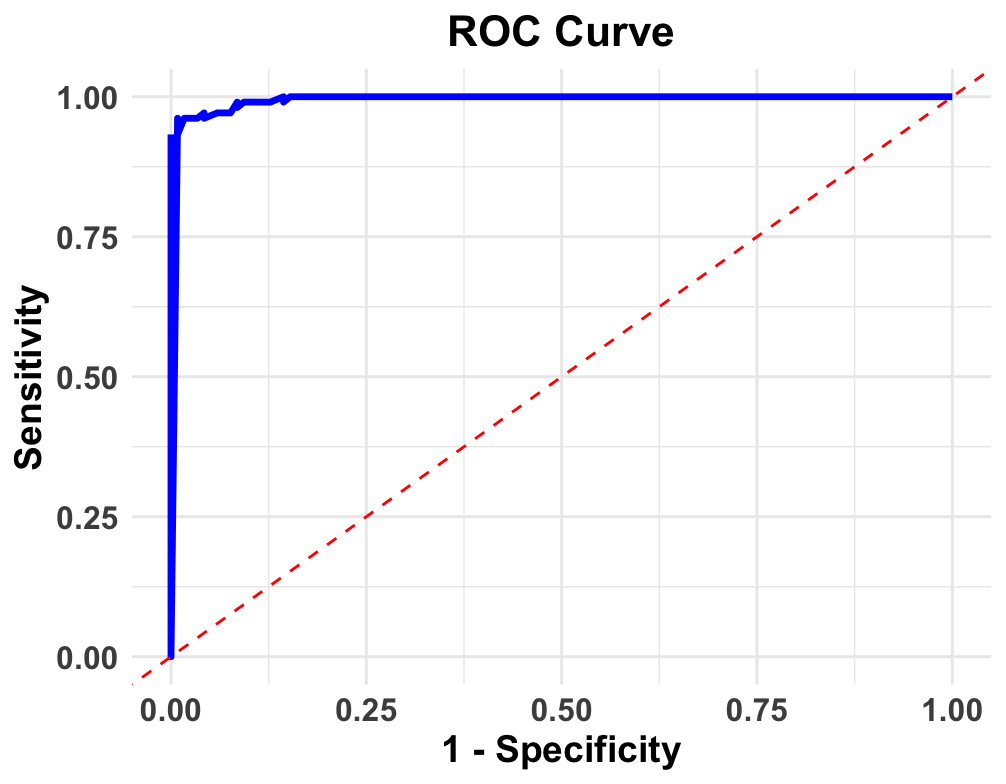
\includegraphics[width=0.9\textwidth]{figures/Random_forest_ROC.png}
    \caption{ROC curve of the Random forest model}
    \label{fig:featureimportance}
\end{figure}

\begin{figure}[H]
    \centering
    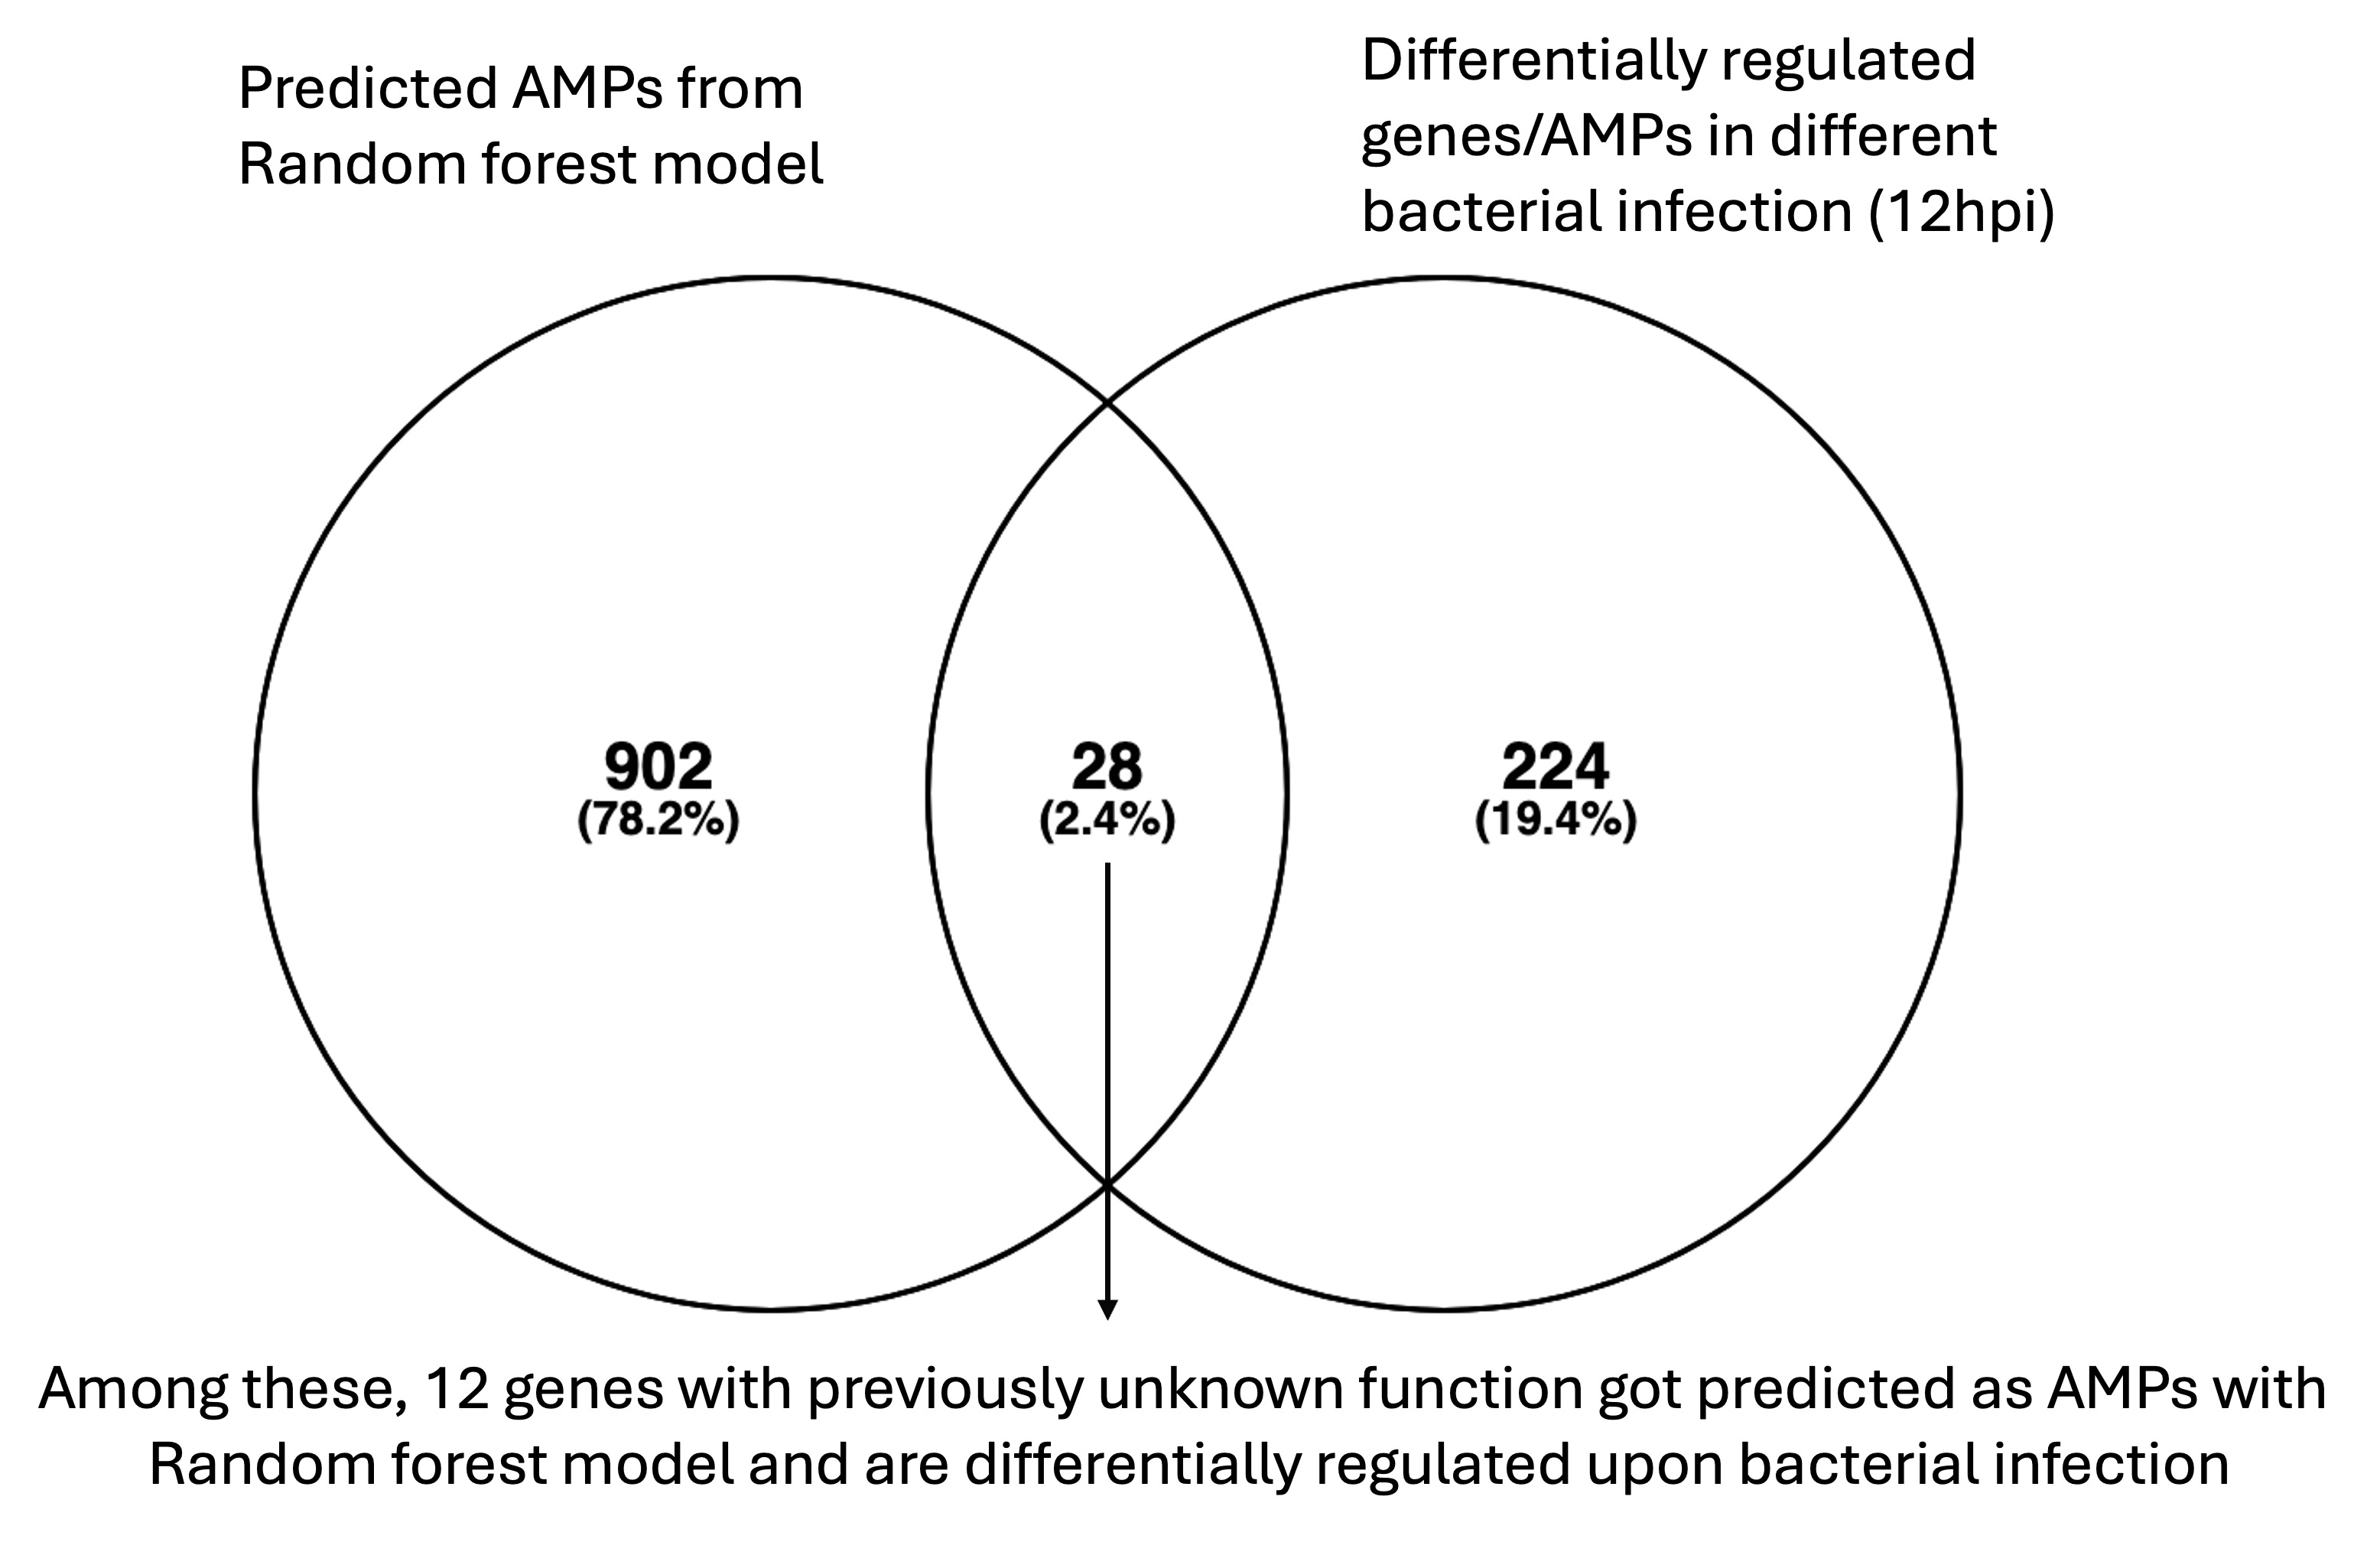
\includegraphics[width=0.9\textwidth]{figures/venn.jpg}
    \caption{Screeing the predicted AMPs with expression data in different bacterial infections}
    \label{fig:featureimportance}
\end{figure}

\begin{figure}[H]
    \centering
    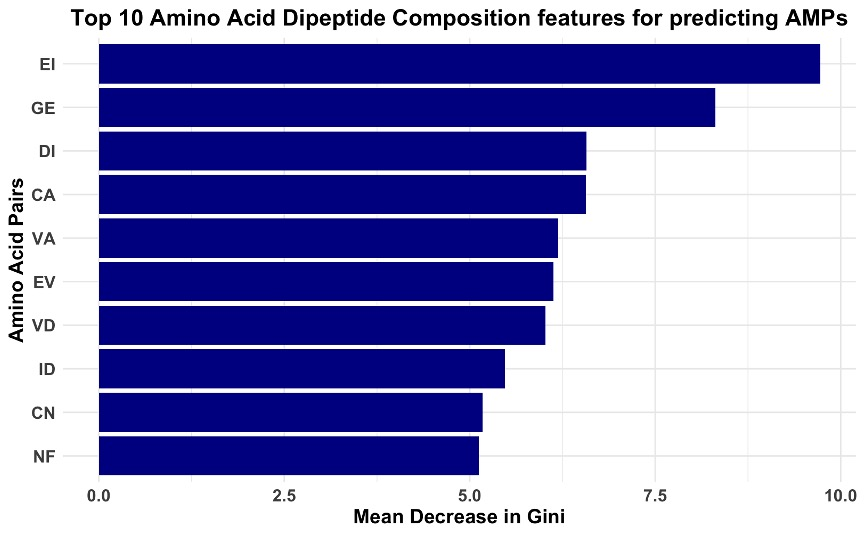
\includegraphics[width=0.9\textwidth]{figures/featureimportance.jpg}
    \caption{Top 10 amino acid dipeptide composition features for predicting AMPs}
    \label{fig:featureimportance}
\end{figure}

%\bibliographystyle{apacite}
%\bibliography{references}

\end{document}